% Architecture diagram of the two-stage recommender.
% Build: pdflatex architecture.tex && pdftocairo -svg architecture.pdf architecture.svg
%        && pdftocairo -png -r 200 -singlefile architecture.pdf architecture
\documentclass{article}
\usepackage[T1]{fontenc}
\usepackage{helvet}
\renewcommand{\familydefault}{\sfdefault}
\usepackage{tikz}
\usepackage{microtype}
\usetikzlibrary{arrows.meta}
\pagestyle{empty}

\definecolor{ink}{HTML}{212529}
\definecolor{muted}{HTML}{495057}
\definecolor{wire}{HTML}{868E96}
\definecolor{datafill}{HTML}{F1F3F5}  \definecolor{dataedge}{HTML}{ADB5BD}
\definecolor{srcfill}{HTML}{E7F0FB}   \definecolor{blue}{HTML}{2A78D6}  \definecolor{blueink}{HTML}{1A4F91}
\definecolor{searchfill}{HTML}{CFE0F6}
\definecolor{rankfill}{HTML}{FFF1E6}  \definecolor{orange}{HTML}{E8590C} \definecolor{orangeink}{HTML}{A63E05}
\definecolor{outfill}{HTML}{EBF7EE}   \definecolor{green}{HTML}{2F9E44}  \definecolor{greenink}{HTML}{1E6B2E}

% \card{title colour}{body colour}{title}{body}
\newcommand{\card}[4]{{\color{#1}\bfseries\normalsize #3}\\[2pt]{\color{#2}\footnotesize #4}}

\tikzset{
  box/.style={rounded corners=5pt, line width=0.9pt, align=center, inner sep=5pt, minimum height=#1},
  box/.default=1.9cm,
  data/.style={box, fill=datafill, draw=dataedge},
  src/.style={box=2.55cm, fill=srcfill, draw=blue},
  rank/.style={box, fill=rankfill, draw=orange},
  result/.style={box=1.6cm, fill=outfill, draw=green},
  wire/.style={draw=wire, line width=0.9pt},
  flow/.style={wire, -{Latex[length=2.6mm, width=2mm]}},
  lane/.style={anchor=west, font=\footnotesize\bfseries, text=wire},
}

\newsavebox{\diagram}
\begin{document}
\sbox{\diagram}{%
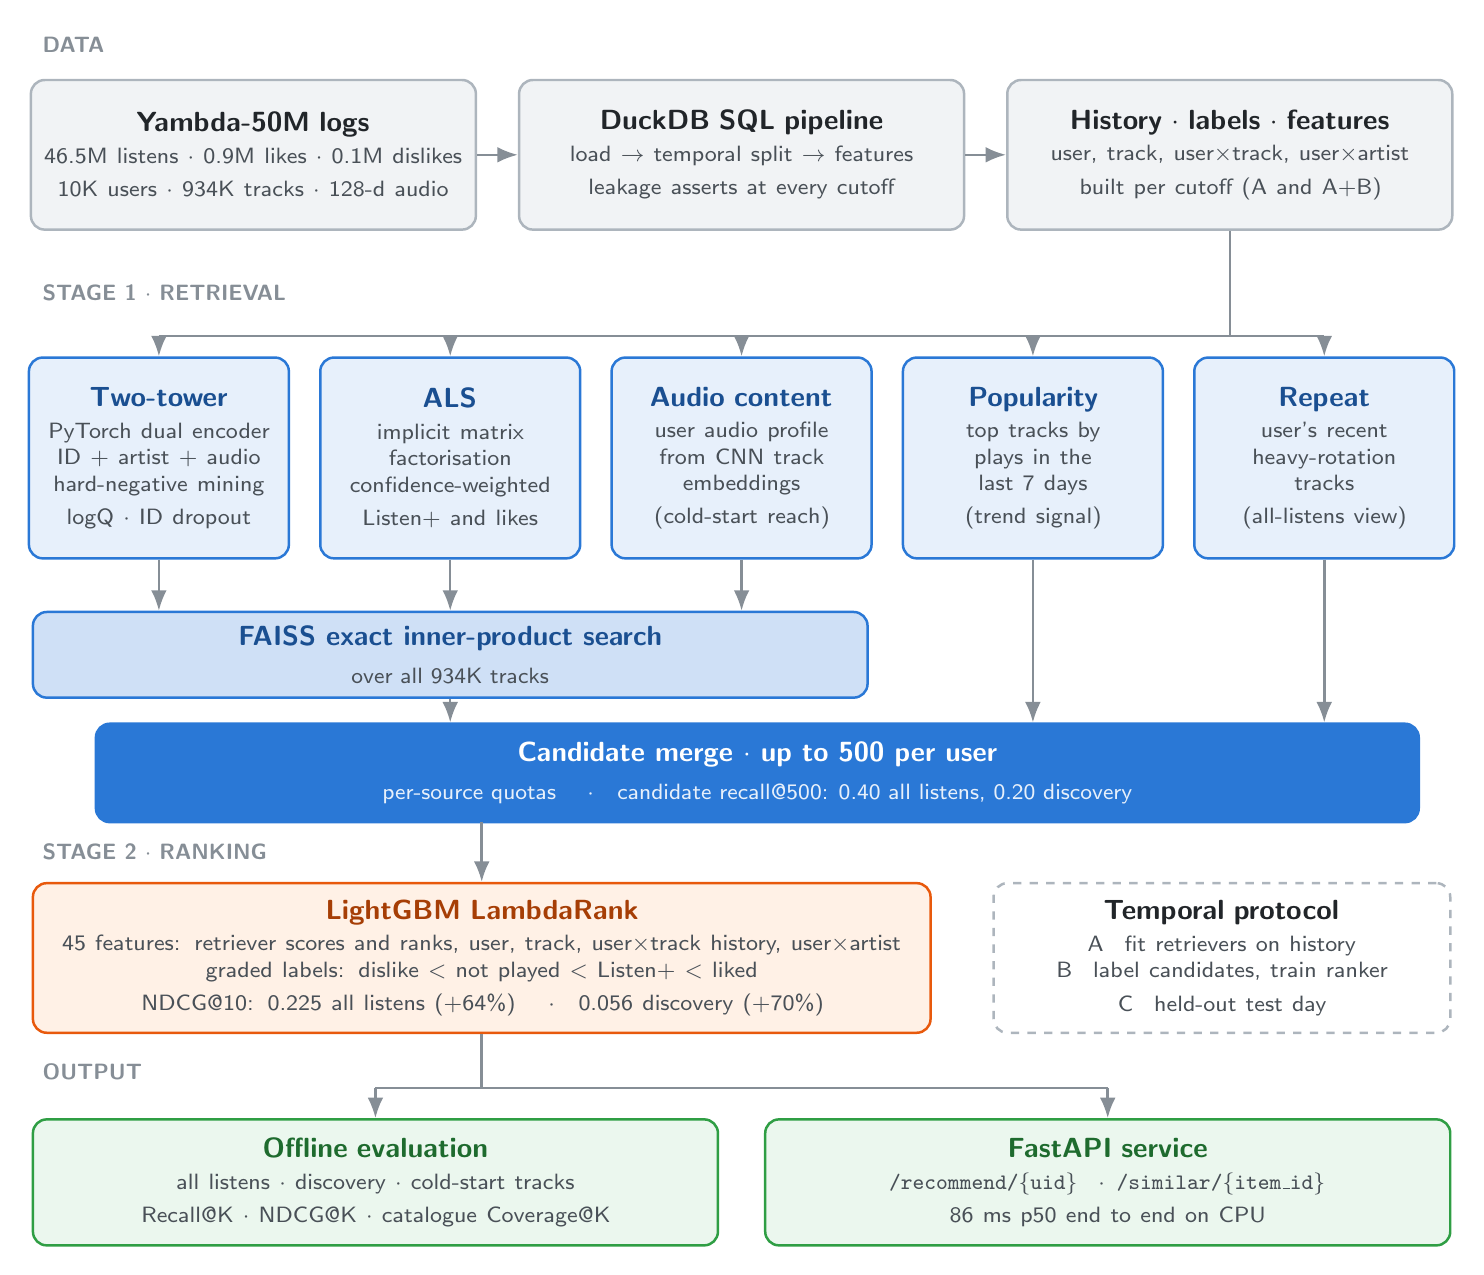
\begin{tikzpicture}[x=1cm, y=1cm]

% ── data ────────────────────────────────────────────────────────────────────────────
\node[lane] at (0, 15.0) {DATA};
\node[data, text width=5.3cm] (raw) at (2.8, 13.6)
  {\card{ink}{muted}{Yambda-50M logs}{46.5M listens $\cdot$ 0.9M likes $\cdot$ 0.1M dislikes\\10K users $\cdot$ 934K tracks $\cdot$ 128-d audio}};
\node[data, text width=5.3cm] (sql) at (9.0, 13.6)
  {\card{ink}{muted}{DuckDB SQL pipeline}{load $\rightarrow$ temporal split $\rightarrow$ features\\leakage asserts at every cutoff}};
\node[data, text width=5.3cm] (feat) at (15.2, 13.6)
  {\card{ink}{muted}{History $\cdot$ labels $\cdot$ features}{user, track, user$\times$track, user$\times$artist\\built per cutoff (A and A+B)}};
\draw[flow] (raw) -- (sql);
\draw[flow] (sql) -- (feat);

% ── stage 1 ─────────────────────────────────────────────────────────────────────────
\node[lane] at (0, 11.85) {STAGE 1 $\cdot$ RETRIEVAL};
\foreach \x/\name/\title/\body in {
    1.6/tt/Two-tower/{PyTorch dual encoder\\ID + artist + audio\\hard-negative mining\\logQ $\cdot$ ID dropout},
    5.3/als/ALS/{implicit matrix\\factorisation\\confidence-weighted\\Listen+ and likes},
    9.0/aud/Audio content/{user audio profile\\from CNN track\\embeddings\\(cold-start reach)},
    12.7/pop/Popularity/{top tracks by\\plays in the\\last 7 days\\(trend signal)},
    16.4/rep/Repeat/{user's recent\\heavy-rotation\\tracks\\(all-listens view)}} {
  \node[src, text width=2.95cm] (\name) at (\x, 9.75) {\card{blueink}{muted}{\title}{\body}};
  \draw[flow] (\x, 11.3) -- (\name.north);
}
\draw[wire] (feat.south) -- (15.2, 11.3);
\draw[wire] (1.6, 11.3) -- (16.4, 11.3);

\node[box=1.0cm, fill=searchfill, draw=blue, minimum width=10.6cm] (faiss) at (5.3, 7.25)
  {\card{blueink}{muted}{FAISS exact inner-product search}{over all 934K tracks}};
\foreach \name in {tt, als, aud} \draw[flow] (\name.south) -- (\name.south |- faiss.north);

\node[box=1.25cm, fill=blue, draw=blue, minimum width=16.8cm] (merge) at (9.2, 5.75)
  {\card{white}{srcfill}{Candidate merge $\cdot$ up to 500 per user}{per-source quotas \quad$\cdot$\quad candidate recall@500: 0.40 all listens, 0.20 discovery}};
\draw[flow] (faiss.south) -- (faiss.south |- merge.north);
\foreach \name in {pop, rep} \draw[flow] (\name.south) -- (\name.south |- merge.north);

% ── stage 2 ─────────────────────────────────────────────────────────────────────────
\node[lane] at (0, 4.75) {STAGE 2 $\cdot$ RANKING};
\node[rank, minimum width=11.4cm, text width=11cm] (rank) at (5.7, 3.4)
  {\card{orangeink}{muted}{LightGBM LambdaRank}{45 features: retriever scores and ranks, user, track, user$\times$track history, user$\times$artist\\graded labels: dislike $<$ not played $<$ Listen+ $<$ liked\\NDCG@10: 0.225 all listens (+64\%) \quad$\cdot$\quad 0.056 discovery (+70\%)}};
\draw[flow] (5.7, 5.125) -- (rank.north);
\node[box, fill=white, draw=dataedge, dashed, minimum width=5.8cm, text width=5.4cm] at (15.1, 3.4)
  {\card{ink}{muted}{Temporal protocol}{A \enspace fit retrievers on history\\B \enspace label candidates, train ranker\\C \enspace held-out test day}};

% ── output ──────────────────────────────────────────────────────────────────────────
\node[lane] at (0, 1.95) {OUTPUT};
\node[result, minimum width=8.7cm, text width=8.3cm] (eval) at (4.35, 0.55)
  {\card{greenink}{muted}{Offline evaluation}{all listens $\cdot$ discovery $\cdot$ cold-start tracks\\Recall@K $\cdot$ NDCG@K $\cdot$ catalogue Coverage@K}};
\node[result, minimum width=8.7cm, text width=8.3cm] (api) at (13.65, 0.55)
  {\card{greenink}{muted}{FastAPI service}{\texttt{/recommend/\{uid\}} \enspace$\cdot$\enspace \texttt{/similar/\{item\_id\}}\\86 ms p50 end to end on CPU}};
\draw[wire] (rank.south) -- (5.7, 1.75);
\draw[wire] (4.35, 1.75) -- (13.65, 1.75);
\draw[flow] (4.35, 1.75) -- (eval.north);
\draw[flow] (13.65, 1.75) -- (api.north);
\end{tikzpicture}}%
% size the page to the picture
\pdfpagewidth=\dimexpr\wd\diagram+24pt\relax
\pdfpageheight=\dimexpr\ht\diagram+\dp\diagram+24pt\relax
\hoffset=-1in \voffset=-1in \oddsidemargin=12pt \topmargin=12pt
\headheight=0pt \headsep=0pt \topskip=0pt \parindent=0pt
\textwidth=\wd\diagram \textheight=\pdfpageheight
\usebox{\diagram}
\end{document}
